\documentclass[11pt]{book}

% Set table of contents depth

\setcounter{tocdepth}{2}

% Set the margins

\usepackage[left=3.5cm,top=3.5cm,right=2.5cm,bottom=3.0cm,a4paper,twoside]{geometry}

% Set one-and-a-half spacing

\usepackage{setspace}
\setstretch{1.5}

% Set font to charter (just remove for default font)

\usepackage[charter]{mathdesign}

% Set chapter style to avantgarde (big grey numbers)
\usepackage{xcolor}
\RequirePackage[avantgarde]{quotchap}

% Load various packages

\usepackage{natbib}
\usepackage{graphicx}
\usepackage{xspace}
\usepackage{lscape}
\usepackage{longtable}
\usepackage{amsmath}
\usepackage{fancyhdr}
\usepackage{titlesec}
\usepackage[breaklinks]{hyperref}
\usepackage{afterpage}
\usepackage[hang,flushmargin]{footmisc} 
\usepackage{todonotes}
\usepackage{epigraph}

% Adding packages for epigraphs.
\setlength\epigraphwidth{1\textwidth}
\setlength\epigraphrule{0pt} % no line between
\setlength\beforeepigraphskip{1\baselineskip} % space before and after epigraph
\setlength\afterepigraphskip{2\baselineskip}
\renewcommand*{\textflush}{flushright}
\renewcommand*{\epigraphsize}{\normalsize\itshape}

% Set caption style

\usepackage[small,bf]{caption}

% Include custom definitions (edit definitions.tex)

\usepackage{xspace}

\newcommand{\eq}{Eq.}
\newcommand{\eqs}{Eqs.}
\newcommand{\fig}{Figure}
\newcommand{\figs}{Figures}

\newcommand{\figshortleft}{{\textit{left}}}
\newcommand{\figshortcenter}{{\textit{center}}}
\newcommand{\figshortright}{{\textit{right}}}

\newcommand{\figleft}{{\textit{Left}}~--~}
\newcommand{\figcenter}{{\textit{Centre}}~--~}
\newcommand{\figright}{{\textit{Right}}~--~}

\newcommand{\figtopleft}{{\textit{Top left}}~--~}
\newcommand{\figtopright}{{\textit{Top right}}~--~}

\newcommand{\figcenterleft}{{\textit{Centre left}}~--~}
\newcommand{\figcenterright}{{\textit{Centre right}}~--~}

\newcommand{\figbottom}{{\textit{Bottom}}~--~}
\newcommand{\figtop}{{\textit{Top}}~--~}

\newcommand{\figbottomleft}{{\textit{Bottom left}}~--~}
\newcommand{\figbottomright}{{\textit{Bottom right}}~--~}

%%%%%%%%%%%%%%%%% Abbreviations %%%%%%%%%%%%%%%%%

\newcommand\tablenotemark[1]{$^{\rm #1}$\xspace}
\newcommand\nodata{$\cdots$}
%----------------- Parameters -------------------

%\newcommand\ion[2]{#1$\;${\small\rmfamily\@Roman{#2}}\relax}%
\renewcommand\line[2]{#1$\;${\small\sc #2}\xspace}%
\newcommand\forbidden[2]{[#1$\;${\small\sc #2}]\xspace}%

%% MATH SYMBOLS %%

\newcommand{\agestar}{t_{\star}}

\newcommand{\mstar}{M_{\star}}
\newcommand{\rstar}{R_{\star}}
\newcommand{\tstar}{T_{\star}}

\newcommand{\mdote}{\dot{M}_{\rm env}}
\newcommand{\rmaxe}{R_{\rm env}^{\rm max}}
\newcommand{\rmine}{R_{\rm env}^{\rm min}}

\newcommand{\mdisk}{M_{\rm disk}}
\newcommand{\mdotdisk}{\dot{M}_{\rm disk}}

\newcommand{\rmaxd}{R_{\rm disk}^{\rm max}}
\newcommand{\rmind}{R_{\rm disk}^{\rm min}}

\newcommand{\rsub}{R_{\rm sub}}

\newcommand{\rhoconst}{\rho_{\rm cavity}}
\newcommand{\thetacav}{\theta_{\rm cavity}}

\newcommand{\rhoamb}{\rho_{\rm ambient}}

\newcommand{\rc}{R_{\rm c}}

\newcommand{\zmin}{z_{\rm factor}}

\newcommand{\msunmath}{M_{\odot}}

\newcommand{\renv}{R_{\rm{env}}}

\newcommand{\fnu}{F_{\nu}}
\newcommand{\rnu}{R_{\nu}}
\newcommand{\fnua}{F_{\nu}{\rm{[actual]}}}
\newcommand{\fnuq}{F_{\nu}{\rm{[assumed]}}}
\newcommand{\fnuqz}{F_{\nu_0}{\rm{[quoted]}}}
\newcommand{\fnuqiso}{F_{\nu_0}^{\rm iso}{\rm{[quoted]}}}

%% UNITS %%

% Temperature

\newcommand{\kelvin}{\,K\xspace}

% Distance

\newcommand{\angstrom}{\,\AA\xspace}
\newcommand{\microns}{\,$\mu$m\xspace}
\newcommand{\mm}{\,mm\xspace}
\newcommand{\rsun}{$R_{\odot}$\xspace}
\newcommand{\au}{\,AU\xspace}
\newcommand{\pc}{\,pc\xspace}
\newcommand{\kpc}{\,kpc\xspace}
\newcommand{\cm}{\,cm\xspace}
\newcommand{\m}{\,m\xspace}

% Time

\newcommand{\seconds}{\,s\xspace}
\newcommand{\days}{\,days\xspace}
\newcommand{\yr}{\,yr\xspace}
\newcommand{\peryr}{\,yr$^{-1}$\xspace}
\newcommand{\Myr}{\,Myr\xspace}
\newcommand{\perMyr}{\,Myr$^{-1}$\xspace}

% Mass

\newcommand{\msun}{\,$M_{\odot}$\xspace}
\newcommand{\msunperyr}{\,$M_{\odot}$\,yr$^{-1}$\xspace}

% Luminosity/Brightness

\newcommand{\lsun}{$L_{\odot}$\xspace}
\newcommand{\mags}{\,mag\xspace}
\newcommand{\Jy}{\,Jy\xspace}
\newcommand{\mJy}{\,mJy\xspace}
\newcommand{\MJysr}{\,MJy/sr\xspace}

% Other

\newcommand{\arcsec}{$^{\prime\prime}$\xspace}
\newcommand{\arcmin}{$^{\prime}$\xspace}
\newcommand{\degrees}{$^\circ$\xspace}
\newcommand{\sqdeg}{\,deg$^2$\xspace}

\newcommand{\gcm}{\,g\,cm$^{-3}$\xspace}

%% MISC %%

%----------------- Spectral indices ----------------

\newcommand{\alpharef}{$\alpha_{[K\,\&\,\rm{MIPS}\,24]}$\xspace}
\newcommand{\alphaend}{$\alpha_{[\lambda_1\,\&\,\lambda_2]}$\xspace}
\newcommand{\alphaall}{$\alpha_{[\lambda_1\,\rightarrow\,\lambda_2]}$\xspace}

%--------------------- Units ---------------------

\newcommand{\mips}{MIPS 24\,$\mu$m\xspace}

\newcommand{\percent}{\,\%\xspace}

%------------------ Quantities -------------------

\newcommand{\hh}{H$_2$\xspace}
\newcommand{\hhmath}{{\rm H}_2}

\newcommand{\rv}{$R_V$}
\newcommand{\av}{A$_{\rm V}$\xspace}
\newcommand{\avmath}{{\rm A}_{\rm V}}

\newcommand{\ks}{K$_{\rm s}$\xspace}

% FITTER PAPER

\newcommand{\lstar}{L_{\rm bol}}
\newcommand{\halpha}{H$\alpha$\xspace}
\newcommand{\irac}{IRAC 8.0\microns}
\newcommand{\msx}{MSX 8.28\microns}
\newcommand{\msxe}{MSX 21.3\microns}
\newcommand{\ratio}{F$_{[{\rm IRAC}~8.0]}$/F$_{[{\rm MSX}~8.28]}$}



% Set page headers
\fancyhead{}
\fancyhead[RO]{\it \nouppercase{\rightmark}}
\fancyhead[LE]{\it \nouppercase{\leftmark}}

% Set headings format

\titleformat{\paragraph}[runin]{}{}{}{\bfseries\em}[:]

% Set headings spacing

\titlespacing*{\section}{0pt}{0.1in}{0.0in}
\titlespacing*{\subsection}{0pt}{0.1in}{0.0in}
\titlespacing*{\subsubsection}{0pt}{0.1in}{0.0in}
\titlespacing*{\paragraph}{0pt}{0.0in}{0.1in}

% Set various lengths

\setlength{\parsep}{0.0in}
\setlength{\topskip}{0in}
\setlength{\topsep}{0.15in}

\setlength{\headsep}{0.20in}
\setlength{\parskip}{0.1in}
\setlength{\partopsep}{0.0in}

\setlength{\floatsep}{0.25in}
\setlength{\textfloatsep}{0.10in}
\setlength{\abovecaptionskip}{0.10in}
\setlength{\belowcaptionskip}{0.00in}

% Figure width and displacement

\newlength{\figwidth}
\setlength{\figwidth}{6.0in}

\newlength{\figmargin}
\setlength{\figmargin}{-0.10in}

\newlength{\initialjump}
\setlength{\initialjump}{-1.00in}

\newcommand\T{\rule{0pt}{3.1ex}}
\newcommand\B{\rule[-1.7ex]{0pt}{0pt}}

\renewcommand{\topfraction}{0.9}
\renewcommand{\textfraction}{0.07}
\setcounter{totalnumber}{1}

% adding text colour options
\newcommand{\red}[1]{{\textcolor{red}{#1}}}
\newcommand{\green}[1]{{\textcolor{green}{#1}}}
\newcommand{\blue}[1]{{\textcolor{blue}{#1}}}

% Start document

\begin{document}
% Make title page
\pagestyle{empty}

\begin{titlepage}
\newcommand{\HRule}{\rule{\linewidth}{0.5mm}}
\center
\vspace*{0.3cm}
\textsc{\LARGE The University of St Andrews}\\[0.1cm] % Name of your university/college
\textsc{\Large School of Physics and Astronomy}\\[3cm] % Major heading such as course name

\includegraphics[width=0.7\textwidth]{thesis/latex/st_a_logo_.png}

\HRule \\[0.4cm]
{ \LARGE Galaxies as potential tracers: \Large \\[0.2cm] \textbf{Looking for halo assembly bias in galaxy observables}}\\[0.4cm] % Title of your document
\HRule \\[1.6cm]
\Large
\textsl{by} \\
\textbf{Christopher James Duckworth}
\\
\vspace*{2cm}
\textsl{\Large Submitted for the degree of Doctor of Philosophy in Astrophsyics}\\[0.6cm] % Minor heading such as course title
{\Large {March 2020}}\\[3cm]
\vfill % Fill the rest of the page with whitespace

\end{titlepage}

\frontmatter

\chapter{Declaration}

I, Christopher James Duckworth, hereby certify that this thesis, which is approximately 50,000 words in length, has been written by me, that it is the record of work carried out by me and that it has not been submitted in any previous application for a higher degree.\\

Date  \hspace{1.8in} Signature of candidate \\

I was admitted as a research student in September 2016 and as a candidate for the degree of PhD in September 2016; the higher study for which this is a record was carried out in the University of St Andrews between 2016 and 2020.\\

Date  \hspace{1.8in} Signature of candidate \\

I hereby certify that the candidate has fulfilled the conditions of the Resolution and Regulations appropriate for the degree of PhD in the University of St Andrews and that the candidate is qualified to submit this thesis in application for that degree.\\

Date  \hspace{1.8in} Signature of supervisor \\

\chapter{Copyright Agreement}

In submitting this thesis to the University of St Andrews we understand that we are giving permission for it to be made available for use in accordance with the regulations of the University Library for the time being in force, subject to any copyright vested in the work not being affected thereby. We also understand that the title and the abstract will be published, and that a copy of the work may be made and supplied to any bona fide library or research worker, that my thesis will be electronically accessible for personal or research use unless exempt by award of an embargo as requested below, and that the library has the right to migrate my thesis into new electronic forms as required to ensure continued access to the thesis. We have obtained any third-party copyright permissions that may be required in order to allow such access and migration, or have requested the appropriate embargo below.\\

The following is an agreed request by candidate and supervisor regarding the electronic publication of this thesis: Access to Printed copy and electronic publication of thesis through the University of St Andrews.\\

Date  \hspace{1.8in} Signature of candidate \\

Date  \hspace{1.8in} Signature of supervisor \\

\setstretch{1.3}

\chapter{Abstract}

All your base are belong to us.

\chapter{Acknowledgements}

All your base are belong to us.

\newpage

\setstretch{1.0}

\tableofcontents

\listoffigures

\listoftables

\setstretch{1.5}

\mainmatter

\pagestyle{fancy}

% NOTE: Here come the chapters - you can have one file per chapter. When you are writing a given chapter, you can always comment out the others to speed up the typesetting.

\chapter{Introduction}
\vspace{-5in}

\includegraphics[height=2.0in]{thesis/latex/st_a_logo_.png}
\vspace{3in}

\label{ch:intro}
The clustering of dark matter haloes is dependent on their constituent masses. This translates observationally into more massive and passive galaxies being more clustered than their lower mass counterparts. The dependence of halo clustering on properties outside of the driving factor of halo mass has been termed `\textit{halo assembly bias}'. Halo spin, concentration and formation time have been found, in simulations, to alter halo clustering, however observationally we are yet to determine whether these are independent or a secondary effect of density and hence halo mass. The motivation of this thesis lies therein. 
\section{Halo assembly bias}
\colorlet{chaptergrey}{orange}
%\renewcommand*\sectfont{\color{orange}}

\chapter[Signatures of halo assembly in kinematically misaligned galaxies]{Signatures of halo assembly in kinematically misaligned galaxies}
\label{ch:kin_mis}
\vspace{-5.25in}
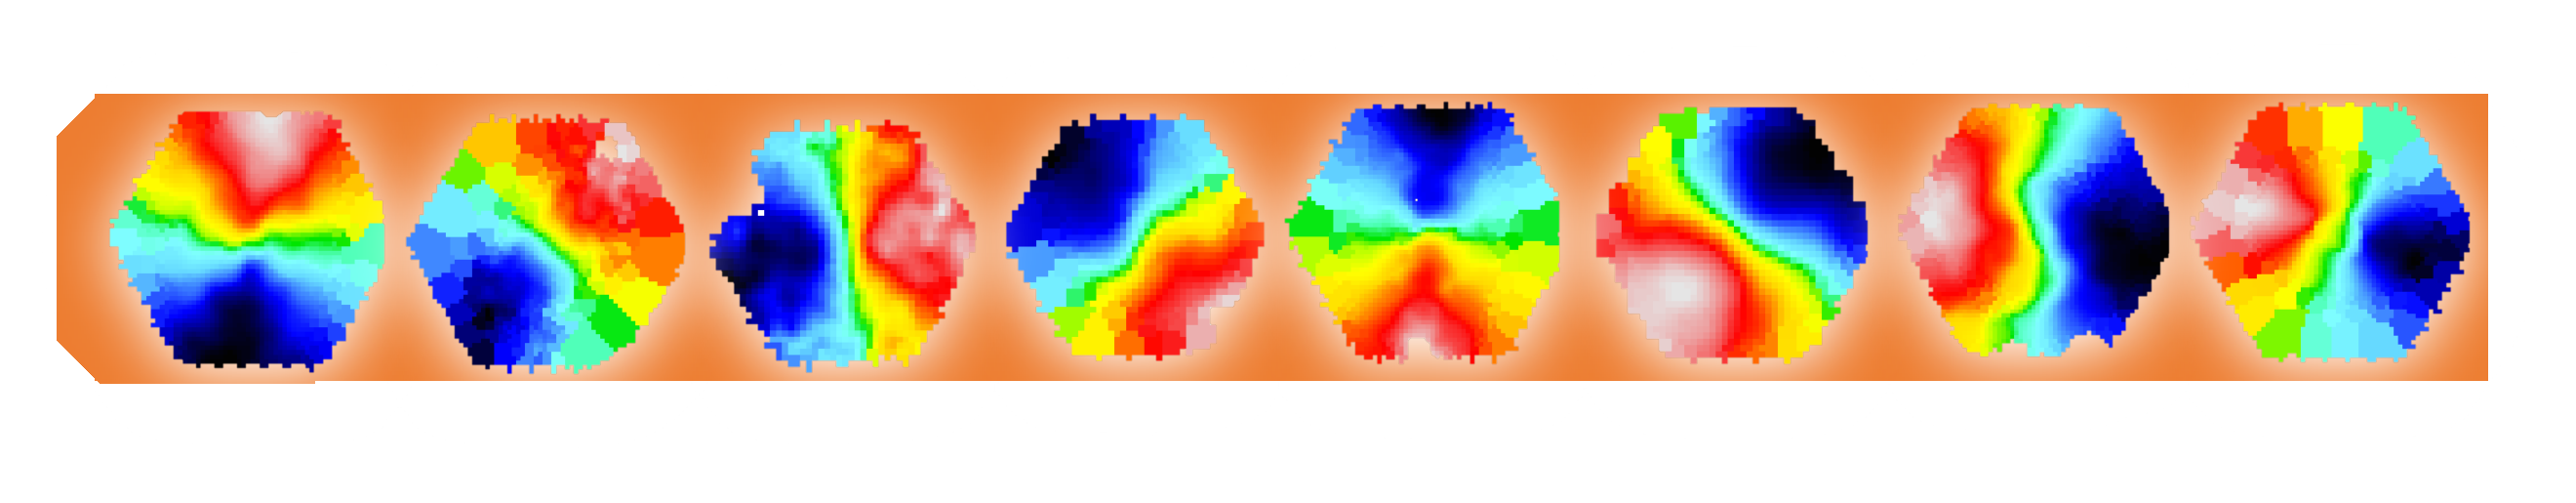
\includegraphics[height=1.39in]{thesis/latex/kin_mis_files/kin_mis_chapter_heading.pdf}
\vspace{3in}

\epigraph{This chapter is based on Duckworth, Tojeiro, Kraljic, Sgr\'o, Wild, Weijmans, Lacerna and Drory, in MNRAS, 448, Issue 1, 2019. Here, we investigate the relationship between kinematically misaligned galaxies with their large-scale environment, in the context of halo assembly.}

\section{Introduction}
Unlike single-fibre galaxy surveys such as SDSS which only obtain spectra from the central $\sim 3 ''$ of a target galaxy, integral field unit (IFU) observations enable spatially resolved spectral measurements up-to several effective radii ($R_{e}$) across the faces of nearby galaxies. The ability to characterise the rotation of stars and ionized gas is a useful indicator of the recent interaction history of a galaxy. Assuming gas that has cooled from stellar mass loss to be kinematically aligned with the original stars, an offset between the rotation of stars and ionized gas is indicative of external gas origin \citep[see][]{sarzi2006,davis2011a}. 

Previous work has focused on the gas content in early-type galaxies (ETGs) and the fraction of which that are significantly kinematically misaligned (i.e. global position angle between rotational directions of gas and stars is greater than 30$^{\circ}$; see \S\ref{sec:kin_mis}) indicating external influence (see. \citet{davis2011a} identify that approximately 36\% of fast-rotating ETGs are kinematically misaligned within the volume-limited sample of ATLAS\textsuperscript{3D} \citep{atlas3d}. \todo{Discussion included here concerns misalignment time-scales - introduce here or later on?}
% This can also be used to constrain the time-scales of misalignment. \citet{davis2016} utilise a toy model to propose that misaligned gas could relax gradually over time-scales of 1-5 Gyr. A faster time-scale of relaxation would require merger rates of $\approx 5$ Gyr\textsuperscript{-1} and hence is disfavoured. The interplay between the strength and persistence of the gas in-flow and the re-aligning torque of the stellar component dictates the exact time-scale of misalignment for an individual galaxy. The strength of a galaxy's stellar torque scales as a function of radius, with the central component of a galaxy re-aligning on a quicker time-scale than the outer regions. 
% The persistence of misalignment has also been considered in numerical simulations. \citet{vdvoort2015} consider the evolution of a misaligned gas disc formed from a merger which removes most of the original disc. During re-accretion of the cold gas, the misaligned disc persists for approximately 2 Gyr before the gas-star rotation angle falls below 20$^{\circ}$. The sustainment of this misalignment is due to continued gas accretion for approximately 1.5 Gyr before its rate falls and the gas can realign with the stellar component on approximately six dynamical time-scales. 

IFU observations are costly, and such detailed information has often come at the cost of total galaxies observed. For example, in the last 10 years ATLAS\textsuperscript{3D} and \red{CALIFA} \citep{califa} observed 260 and 667 galaxies respectively with various selection criteria. To characterise the impact of halo assembly bias and cosmic web environment on galaxy kinematics, we are looking for second order effects (after the driving force of stellar mass) and hence require large sample sizes to decompose signal. 

At the present-time, however, there are two large-scale IFU surveys which could provide a sample large enough for a statistically significant characterisation with respect to halo assembly or environment. The Sydney-AAO Multi-object Integral field spectrograph survey \citep[SAMI;][]{croom2012,bryant2015} will map $\sim$3400 galaxies in the local universe ($z < 0.12$) across a large range of environments in the GAMA footprint. In parallel, the Mapping Nearby Galaxies at Apache Point \citep[MaNGA;][]{bundy2015,blanton2017} survey will map $\sim$10000 galaxies up to $z = 0.15$, with the aim of creating a sample with near flat number density distribution in absolute $i$-band magnitude and stellar mass. The preceding work in this Chapter and \todo{add chapters here.}, is based on data from the MaNGA survey and investigates the relationship between kinematic misalignment in galaxies and their large-scale environment, in the context of halo assembly. 

\red{The impact of environment on kinematically misaligned galaxies has been previously studied in MaNGA. Using a sample of 66 misaligned galaxies, \citet{jin2016} found that the fraction of misalignment varies with galaxy properties such as stellar mass and sSFR. Regardless of sSFR, they find that kinematically misaligned galaxies are typically more isolated. Could these correspond to the later forming haloes?}

We explore whether position with respect to filamentary structures identified in the cosmic web, halo age and estimated group occupancy correlate with more recent accretion observed on the central galaxy of the group. A younger halo corresponds, by definition, to more recent dark matter accretion and a richer recent merger history. We explore the idea that low-mass haloes have their cold flow accretion halted due to large-scale tidal environment as indicated by the halo age or vicinity to cosmic web features. We also discuss the prevalence of gas cooling from the hot halo in interpretation of our results and consider the ability of the global position angle to identify gas accretion.

\section{Data}
\subsection{MaNGA}
MaNGA is one of three programs in the fourth generation of the Sloan Digital Sky Survey (SDSS-IV). Using the 2.5-metre telescope at the Apache Point Observatory \citep{gunn2006} along with the two channel BOSS spectrographs \citep{smee2013} and the MaNGA IFUs \citep{drory2015}, MaNGA provides spatial resolution on kpc scales (2'' diameter fibres) while covering 3600-10300$\mathring{A}$ in wavelength with a resolving power of R$\sim$2000. 

By design, the complete sample is unbiased towards morphology, inclination, colour and stellar mass. This is enabled by three major observation subsets: the Primary sample, the Secondary sample and the Colour-Enhanced supplement. All sub-samples observe galaxies to a minimum of $\sim 1.5 R_{e}$ with the Secondary sample increasing this minimum to $\sim 2.5 R_{e}$. The Colour-Enhanced supplement fills in gaps of the colour-magnitude diagram leading to an approximately flat distribution of stellar mass. A full description of the MaNGA observing strategy is given in \citet{law2015obs,yan2016obs}.

% Include a figure showing the distribution of NSA, MaNGA targets, MPL-6 and MPL-8.
% Also include figure of bundle sizes?
MaNGA observations are covered plate by plate, employing a dithered pattern for each galaxy corresponding to one of the 17 fibre-bundles of 5 distinct sizes. MaNGA targets are taken from an adapted version of the NASA-Sloan Atlas (NSA) catalogue. While this selection is naturally not volume limited, it is a simple exercise to correct for since every galaxy in the redshift range is known \citep{wake2017}. Data is provided by the MaNGA data reduction pipeline as described in \citet{law2016drp,yan2016spec}. Any incomplete data release of MaNGA should therefore be unbiased with respect to IFU sizes and hence a reasonable representation of the final sample scheduled to be complete in 2020. 

In this chapter, we use 4633 unique galaxy observations corresponding to the 6th MaNGA product launch (MPL). This reflects the completion of the survey as of mid-2018 (data released publicly December 2018).

\subsection{Velocity fields}
The MaNGA Data Analysis Pipeline \citep[DAP][]{westfall2019,belfiore2019} provides science-ready processed data for MaNGA observations. Some example outputs include; spaxel-by-spaxel coordinate information based on the isophotal ellipticities from the NASA-Sloan Atlas, S/N measurements, binned spectra, stellar kinematics and stellar-continuum models, emission-line properties and models and spectral-index measurements. Kinematics are easily accessible as 2D maps which we use for stellar and gas velocity fields in the following analysis. A complete discussion can be found in \citet{westfall2019,belfiore2019}, however we will summarise the key points concerning stellar and gas velocity fields here.

Stellar kinematics are derived using the Penalised Pixel-Fitting (pPXF) method \citep{cappellari2004,cappellari2017}. This extracts the line of sight velocity dispersion and then fits the absorption-line spectra from a set of 49 clusters of stellar spectra from the MILES stellar library \citep{sanchez2006,falcon2011}. Before extraction of the mean stellar velocity, the spectra are spatially Voronoi binned to $g$-band \textit{S/N} $\sim$ 10, excluding any individual spectrum with a $g$-band \textit{S/N} < 1 \citep{cappellari2003}. This approach is geared towards stellar kinematics as the spatial binning is applied to the continuum \textit{S/N}, however, we note that unbinned and Voronoi binned velocity maps produce similar results when calculating average rotation.

Gas velocity fields are extracted through fitting a Gaussian to the H$\alpha$-6564 emission line, relative to the input redshift for the galaxy. This velocity is representative for all ionized gas, since the parameters for each Gaussian fit to each emission line are tied during the fitting process. These velocities are also binned spatially by the Voronoi bins of the stellar continuum.

\subsection{Kinematic misalignment} \label{sec:kin_mis}
We estimate the two dimensional global position angle (PA) of the stellar and H$\alpha$ gas velocity fields using the \texttt{FIT\_KINEMATIC\_PA} routine outlined in Appendix C of \citet{krajnovic2006}. By default this finds the angle corresponding to the bisecting line which has greatest velocity change along it (i.e. the angle of peak rotational velocity). We choose this angle to be found from sampling at 180 equally spaced steps. This is measured counter-clockwise from the north axis, however, it does not discriminate between the blueshifted and redshifted side since it is only defined up to 180$^{\circ}$. As a result, velocity fields with a difference of 180$^{\circ}$ PA would appear to be aligned. To solve this we identify the direction of rotation and re-assign a consistent PA: defined as the axis of rotation approximately 90$^{\circ}$ clockwise from the blueshifted side. This angle now spans 360$^{\circ}$ allowing an automatic detection of misaligned gas and stellar components. The offset angle between kinematic components is defined as: 
\begin{equation} \label{eq:delPA}
\Delta PA = |PA_{stellar} - PA_{H\alpha}|. 
\end{equation}
We define galaxies with $\Delta$PA > 30$^{\circ}$ to be significantly kinematically misaligned. An example of an aligned and a misaligned galaxy is shown in Figure \ref{fig:cutout_wIFU}. 

\begin{figure*}
	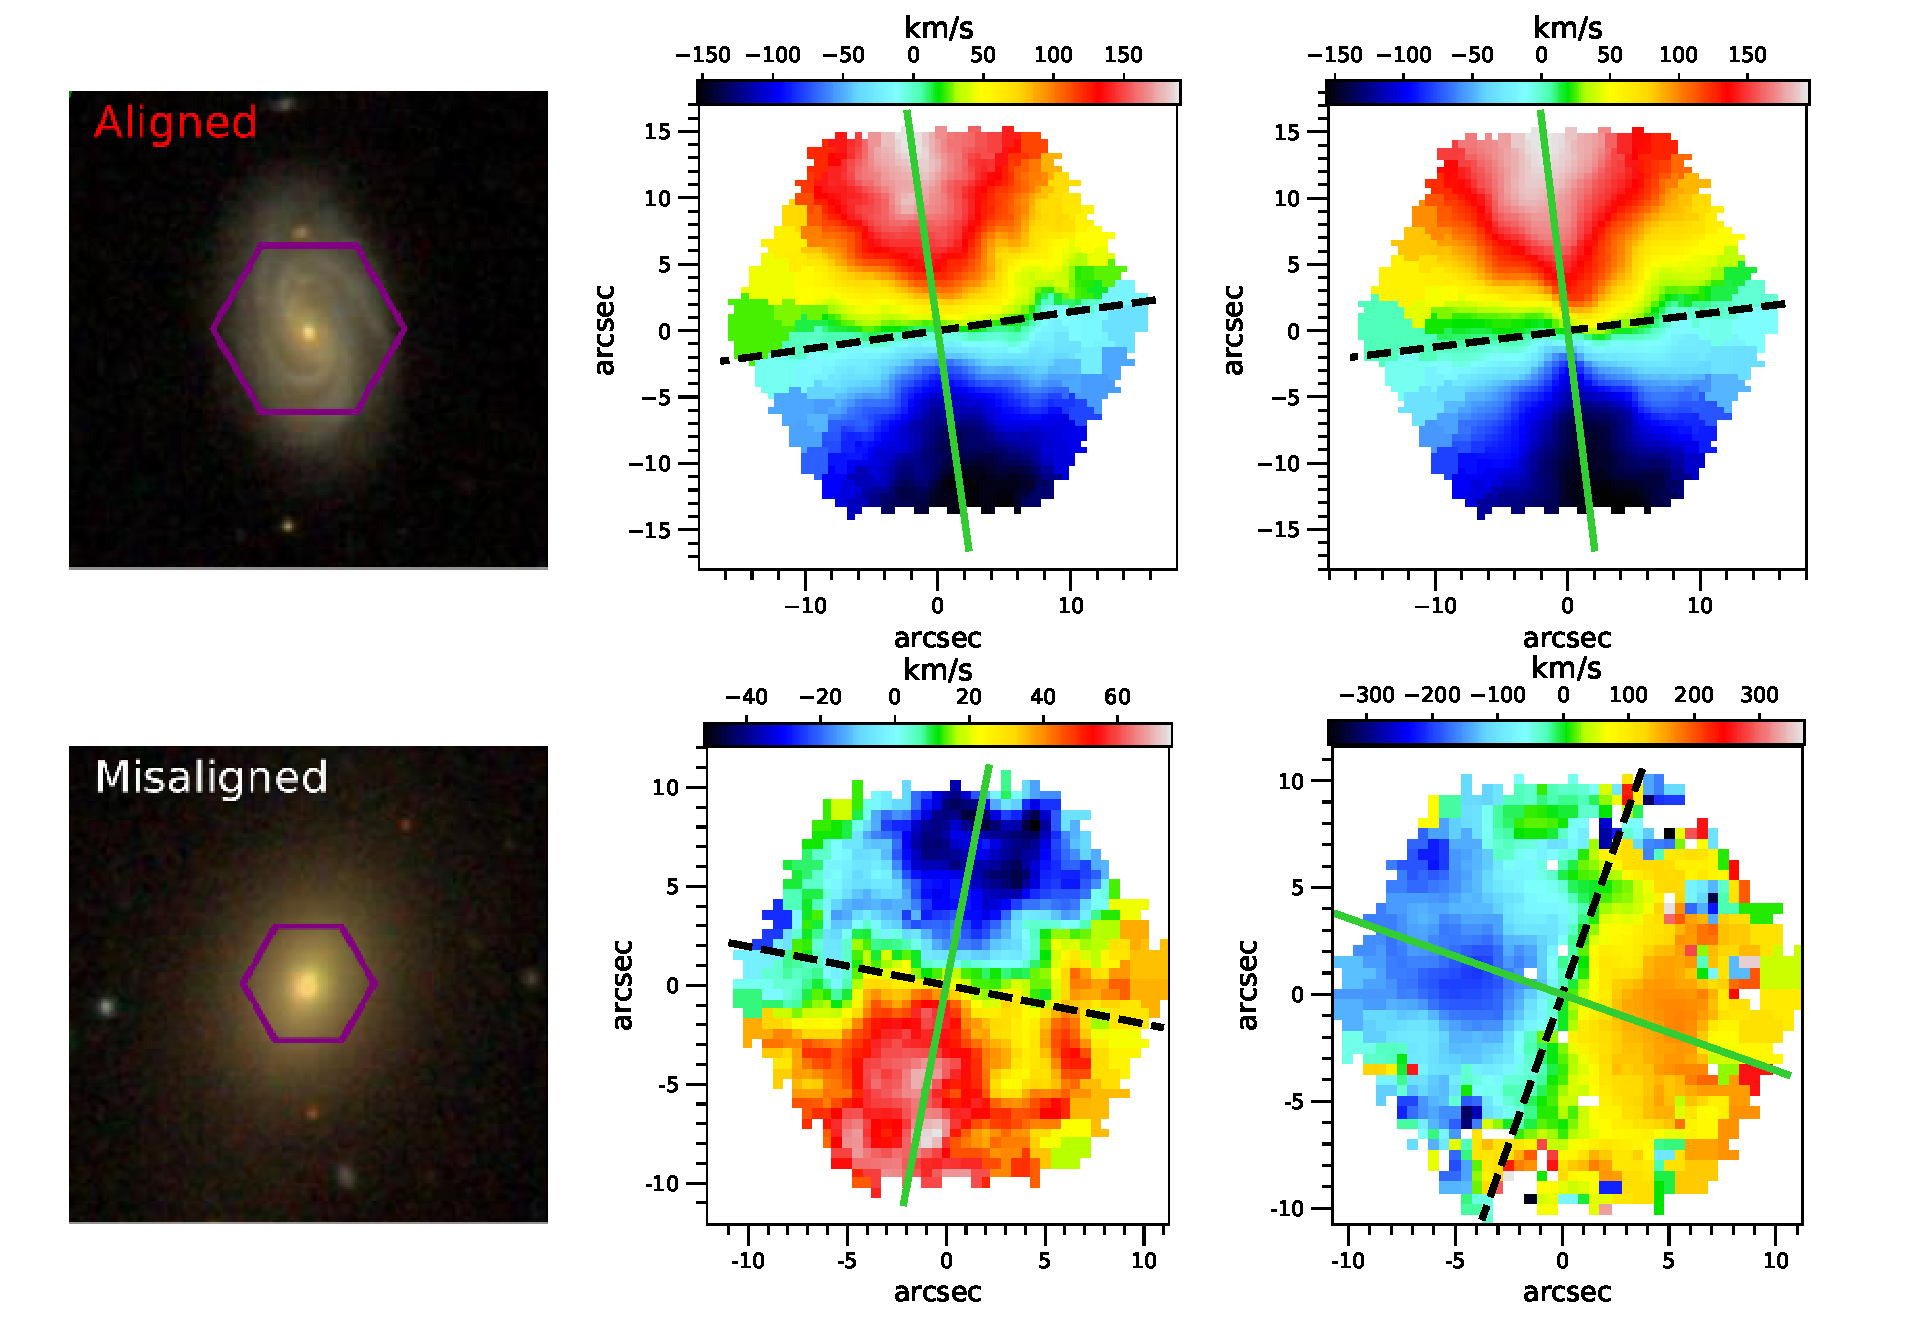
\includegraphics[width=\linewidth]{thesis/latex/kin_mis_files/cutout_wIFU_revised.pdf}
    \caption{Examples of a kinematically aligned (top) and misaligned (bottom) galaxy defined by $\Delta$PA. From left to right, the panels show (i) the original SDSS cutout of surrounding field with the MaNGA IFU footprint overlaid in purple, (ii) stellar velocity field and (iii) $H\alpha$ (gas) velocity field. The velocity fields are marked by a defined PA (green solid line) and axis of rotation (black dashed line). The galaxy in the bottom row is misaligned due to it having $\Delta$PA > 30$^{\circ}$. The colour-bars represent the velocity fields in km/s and the galaxies are orientated so that up corresponds to North and right to East.}
    \label{fig:cutout_wIFU}
\end{figure*}

To improve the reliability of the PA fit, we apply a few additional filters to the velocity fields. While foreground stars are flagged within observations, background/small neighbouring galaxies can remain within the IFU footprint. This is a problem for fitting a global position angle since it naturally interprets other material as part of the target galaxy's observation and interpolates between the regions. We remove all disconnected regions smaller than $10\%$ of the target galaxy's footprint. In addition we sigma clip the velocity field and remove all spectral pixels (spaxels) above a $3\sigma$ threshold.

Our choice to take $\Delta$PA > 30$^{\circ}$ as significantly kinematically misaligned is a conservative selection to ensure we are selecting galaxies undergoing external interaction. There is evidence to suggest that accretion drives misalignment past $\Delta$PA = 30$^{\circ}$. \citet{lagos2015} found that using solely galaxy mergers as the source for misaligned cold gas only predicts 2\% of ETGs to have $\Delta$PA > 30$^{\circ}$ using GALFORM, in comparison with the misaligned field ETG fraction found in ATLAS\textsuperscript{3D} of 42 $\pm$ 6\%  \citep{davis2011a}. This puts a lower level of importance on gas accretion. Our choice can be justified as follows. Firstly, we are using ionized gas as a proxy for the distribution and accretion of cold gas. \citet{davis2011a} find that the typical difference between the PAs of cold gas (CO) and ionized gas can be described by a Gaussian distribution centred on 0 with a standard deviation of 15$^{\circ}$ for 38 CO bright galaxies in ATLAS\textsuperscript{3D}. While indicating ionized gas is a reasonable estimator for cold gas, splitting $\Delta$PA = 30$^{\circ}$ accounts for the scatter in this relationship. Secondly, this should avoid spurious misalignments arising from errors in the fit of $\Delta$PA. While our model errors are low, they are likely an underestimation since they do not include more complex motions. However, selecting a lower split in $\Delta$PA would only be affected by the increased likelihood of internal processes being dominant, rather than the inaccuracy of fitting. Any threshold in $\Delta$PA becomes a trade off between sample size and contamination probability. Altering our cut in $\Delta$PA to be 20$^{\circ}$, 40$^{\circ}$ or similar does not change any of the conclusions drawn in this chapter.

\subsubsection{Error estimation}
We construct two component model velocity maps for each stellar and gas component of every MPL-6 observation in order to estimate typical errors on $\Delta$PA from \texttt{FIT\_KINEMATIC\_PA} for the MaNGA sample. It is an important point to constrain the errors of our PA fits, so we can reliably trust cuts in $\Delta$PA to select galaxies which are significantly kinematically misaligned and hence have had external interaction.

Errors using the \texttt{FIT\_KINEMATIC\_PA} routine have been previously estimated for molecular gas velocity fields in ATLAS\textsuperscript{3D} \citep{davis2011a}. Model velocity fields with a known PA were constructed using an empirical galaxy rotation curve and combined with Gaussian noise matched to the signal-to-noise ratio of the data. A typical scatter of $\approx10^{\circ}$ was found due to varying inclination and angular resolution for the velocity fields.

\subsubsection{Circular velocity}
To find the typical error on $\Delta$PA for galaxies in MaNGA, we create model velocity maps for both the stellar and gas components of each MPL-6 observation. In each instance the basic construction of the model follows Section 4 of \citet{krajnovic2006}. Each velocity field comprises of a two-component Hernquist potential which provides a basic circular velocity given by,
\begin{equation}
V_c = \frac{\sqrt{GMr}}{r+r_0}
\end{equation}
where $G$ is the gravitational constant, $M$ is the total mass and $r_0$ is the core radius of each component respectively \citep{hernquist1990}. We use a two-component model to include the relative strengths of both disc and bulge each with distinct effective radii, $R_e$. We fix $r_0$ to be 5 and 15 (units: $arcsec$) and $\sqrt{GM}$ to be 850 and 1500 (units: $km s^{-1} arcsec^{1/2}) $ for the bulge and disc components respectively. These individual components are light weighted by model sersic flux profiles according to,
\begin{equation}
I(r) = I_0 e^{-\left(\frac{R}{R_e}\right)^{n_s}}
\end{equation}
where $I_{0}$ is the peak flux and $n_s$ is the sersic index which is set to 1 and 4 for the disc and spheroidal components respectively. Since we do not have bulge-disc decompositions, we lack individual effective radii for both the bulge and disc components. Instead, we set the bulge and disc effective radii to be 0.5$R_e$ and 1.5$R_e$, where $R_e$ is the effective radius estimated by an elliptical petrosian fit taken from the NSA targeting catalogue. 

\subsubsection{Calibration}
For each MaNGA galaxy a basic velocity field model is constructed using this template. The axes of the model velocity field are then scaled according to the inclination, $i$, which is estimated from the $b/a$ ratio taken from the NSA catalogue and is also used to scale the fraction of rotational velocity along the line-of-sight. The velocity field for each component, ($j=bulge,disc$), in polar coordinates $(r,\phi)$ is then described by,
\begin{equation}
V(r,\phi) = \frac{I_{j}(r)}{I_{tot}(r)}V_{c}(r)\cos(\phi+\theta_{j})\sin(i)
\end{equation}
where $\theta_j$ is the input kinematic position angle. We set $\theta_{bulge} = \theta_{disc}$ for simplicity, however, we do note that galaxies with more complex orbital motions may increase the typical error. The position angle for both bulge and disc is simply taken to be the opening angle of the galaxy (direction of major axis taken from NSA catalogue). 

In order to imitate a MaNGA observation, the model velocity field is sampled at the spatial resolution of the corresponding IFU bundle and projected into the original shape of the actual observation for H$\alpha$ and stellar maps respectively. Gaussian noise is drawn for each spaxel from a normal distribution with the standard deviation taken from the errors on the actual observation. In addition, these model velocity fields are then Voronoi binned to match the original observation.

Example stellar and H$\alpha$ velocity fields generated from these models are shown in Figure \ref{fig:sim_ifu} with comparison to the actual observation. As expected, the model velocity fields frequently recreate observations well but struggle to encompass more complex motion. For this reason, our models should make a reasonable prediction on the typical $\Delta$PA errors intrinsic to MaNGA observations.

\begin{figure}
	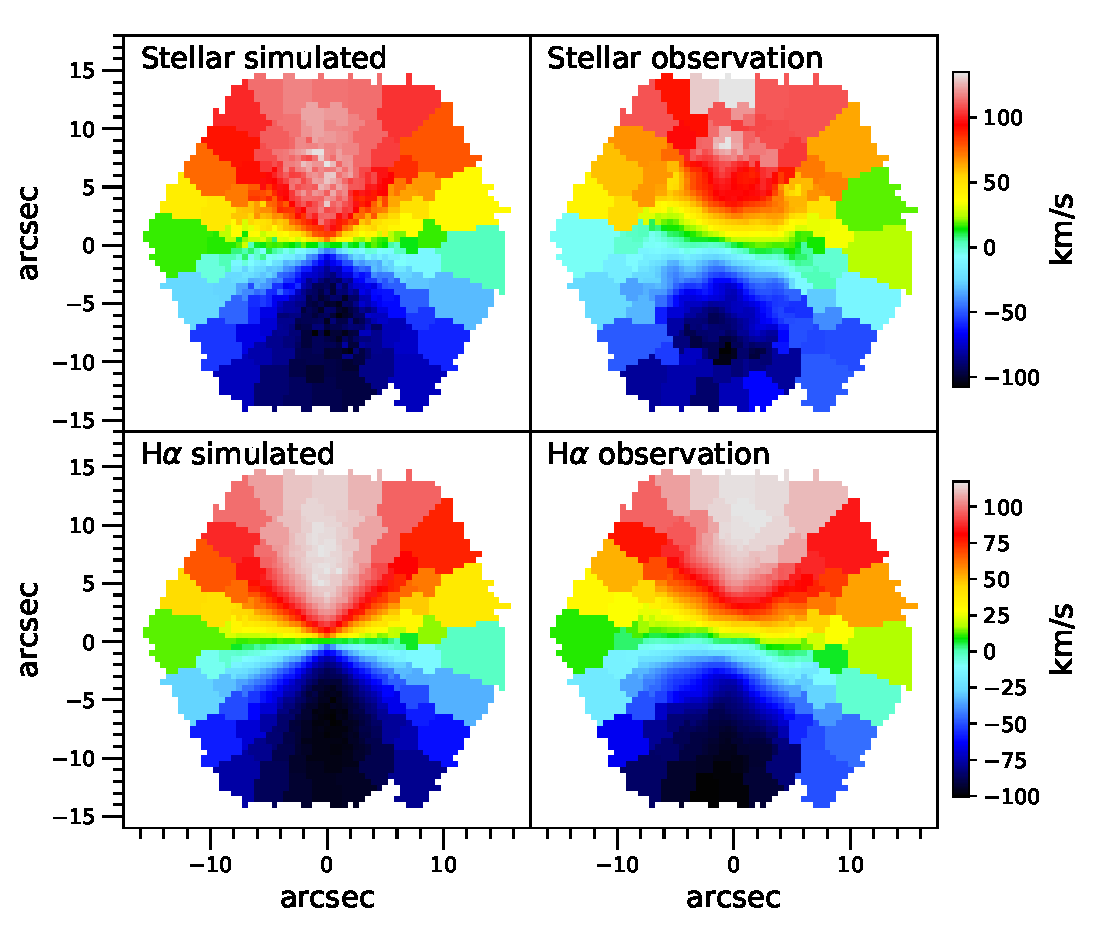
\includegraphics[width=\linewidth]{thesis/latex/kin_mis_files/obs_sim_IFU.pdf}
    \caption{Comparison velocity maps for simulation (left column) and observation (right column). Stellar (H$\alpha$) component velocity maps are shown on the top (bottom) row with the associated velocity colourbars.}
    \label{fig:sim_ifu}
\end{figure}

\subsubsection{Typical errors}
We construct model velocity fields for all non-critically flagged MPL-6 galaxies, inclusive of the $\Delta$PA sample used in this work. Figure \ref{fig:model_errors} shows the cumulative probability distribution for the range of $0-5^{\circ}$ where the majority of errors fall. We find that \texttt{FIT\_KINEMATIC\_PA} gives a typical combined (stellar and gas) mean error of $1.3^{\circ}$. While this is an underestimation of true $\Delta$PA errors for a sample of galaxies including those with more complex velocity fields, it is indicative that selecting a cut at $\Delta$PA = 30$^{\circ}$ should be robust to identifying galaxies with external interaction. \todo{Has python version of fit kinematic pa been updated to include this?}

\begin{figure}
	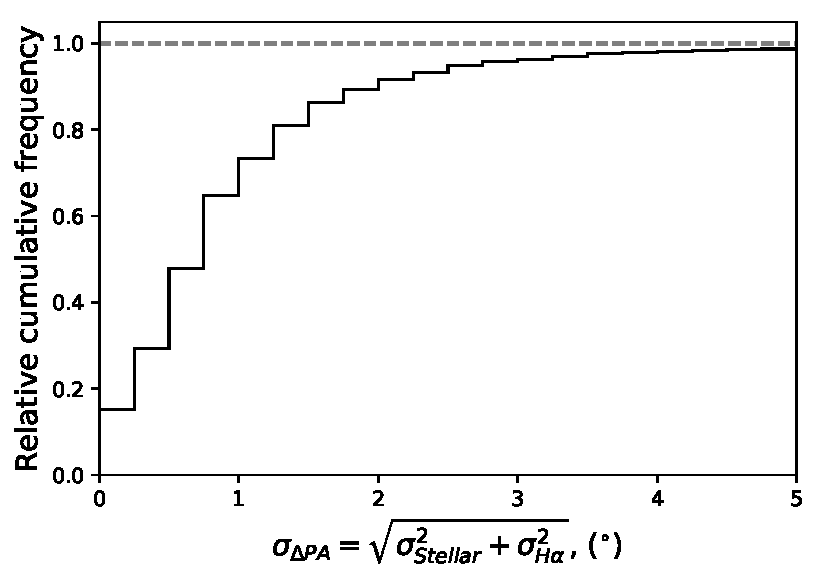
\includegraphics[width=\linewidth]{thesis/latex/kin_mis_files/cumulative_model_errors.pdf}
    \caption{Cumulative histogram of errors for fitting kinematic PA to model maps for the all non-critically flagged MPL-6 galaxy observations.}
    \label{fig:model_errors}
\end{figure}

\subsection{Stellar mass and halo mass definitions}
To analyse the incident effects onto central galaxies as a function of environment, we require individual stellar mass, group identification and estimations of the total halo mass. We use stellar masses estimated in the New-York University Value Added Catalogue from the K-correct routine \citep[NYU-VAC;][]{blanton2005}. \citet{yang2007} (Y07 hence-forth) present an adaptive group finding algorithm based on the NYU-VAC to assign galaxies to haloes and then estimate and revise group properties through iteration. We will summarise the basic steps here. Potential group centres are first found through a friend-of-friends algorithm with small linking lengths in redshift space. All galaxies not currently linked are also considered as potential centres. For each tentative group, the combined luminosity of all group members with 
\begin{equation}
^{0.1}M_r - 5log(h) \leq -19.5
\end{equation}
are found, where $^{0.1}M_r$ is the absolute magnitude estimated from the NYU-VAC K-corrected to $z=0.1$. All galaxies within SDSS data-release 7 (DR7, all spectroscopic galaxies) below $z=0.09$ meet this criteria and hence the combined luminosity can be estimated directly. A corrective factor is applied for groups above this redshift. This total luminosity is then used to assign halo mass and various other group properties, which in turn refines the group identification following an iterative process until conversion. 

We remove all groups with $f_{edge} < 0.6$ as recommended by Y07 corresponding to groups on the survey borders. \citet{yang2009} provide a conservative estimate on the minimum halo mass for groups that would be expected to be complete as a function of redshift. This work primarily focusses on low-mass haloes, ($M_h \lesssim 10^{12.5} M_{\odot}$), however many of these groups will be incomplete at the redshift range selected. Y07 note however that any potential scatter arising from the incompleteness correction should be minimal in comparison with the scatter between group luminosity and assigned halo mass. 

The use of a group catalogue brings important considerations. In low-mass groups, the multiplicity of each group is low, and the luminosity (or stellar mass) of the central galaxy, will largely determine the mass of the group, potentially leading to an under-estimation of the scatter in the stellar-mass to halo-mass relation (see e.g. \citealt{campbell2015, reddick2013}). On the other hand, the fraction of groups with at least one satellite galaxy that is more massive than the central, increases steeply with halo mass (see e.g. \citealt{reddick2013}), leading to artificially larger scatter and an increased likelihood of central misclassification with increasing halo mass. \citet{campbell2015} demonstrate that group finder inferred measurements tend to equalise the properties of distinct galaxy sub-populations, however in general it is possible to recover meaningful physical correlations for average properties as a function of stellar and halo mass. 

We select only galaxies classified as centrals corresponding to the most massive galaxy within each group identified by Y07. The relationship between the central stellar mass and halo mass for galaxies within Y07 is shown in Figure \ref{fig:stel_halo_dist}. The increase of scatter in this relationship with increasing halo mass is likely explained by the limitations of group catalogues mentioned above. 

\begin{figure}
	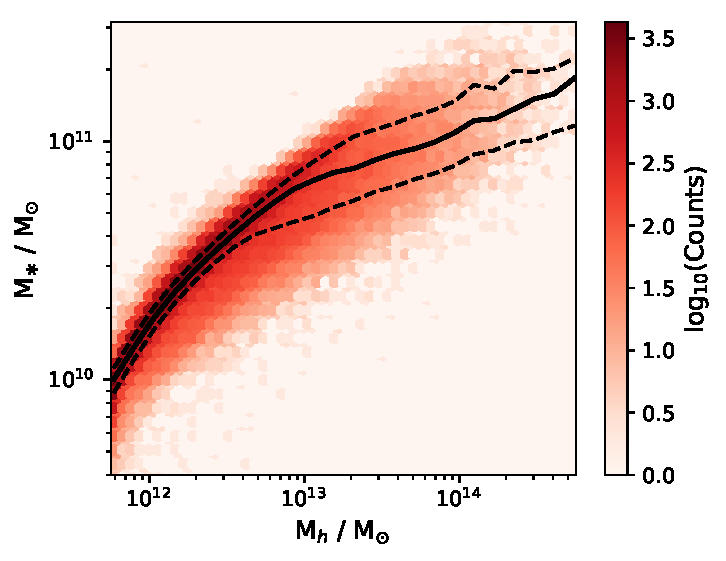
\includegraphics[width=\linewidth]{thesis/latex/kin_mis_files/stel_halo_ratio_dist.pdf}
    \caption{Hexagonal density plot of the relationship between the stellar mass  and the halo mass for central galaxies within Y07. The number counts are scaled logarithmically. The black lines show the median (solid) and the 20th and 80th quantiles (dashed) of the stellar mass in bins of halo mass.}
    \label{fig:stel_halo_dist}
\end{figure}

\section{Sample selection} \label{sec:samp_sec}
While the complete MaNGA sample may be unbiased to morphology, we must proceed with care when selecting a sub-sample usable for kinematic disturbance. To remove spurious PA fits we eyeball the entire MPL-6 sample and remove all galaxies which have a largely incomplete velocity field, poor or biased PA fit or are virtually face-on so that little or no rotational component is along the line of sight. This removes approximately half of MPL-6 observations. The majority of galaxies removed have largely incomplete gas velocity fields and for that reason our analysis naturally excludes gas-poor and slowly rotating elliptical galaxies. 

Recent studies have found that the fraction of slow rotators increases steeply with stellar mass and has a weak dependence on environment once this is controlled for \citep[e.g.][]{greene2018,lagos2018}. We note that our natural exclusion of gas-poor high-mass galaxies is reflected in the stellar mass distribution of the $\Delta$PA defined sample in Figure \ref{fig:samp_cons}. \todo{Add sample selection figure - should combine MPL-6 to MPL-8 ? }

GalaxyZoo1\footnote{At the point of submission for this work, GalaxyZoo1 provided the largest sample of galaxies with classified morphologies for the MaNGA survey. Since then a complete catalogue for all MaNGA targets has been constructed which will be used and described in \red{Chapter...}} provides visually identified morphologies for a large sample of SDSS galaxies \citep{lintott2008}. Morphology is identified by having over 80\% of debiased classification votes in the same category (i.e. elliptical or spiral). The remainder of galaxies are marked as uncertain morphology. We compare the fraction of ellipticals in our $\Delta$PA sub-sample with MPL-6, as shown in Table \ref{tab:GZ}. GalaxyZoo1 only provides classifications for 3/4 of MPL-6 as reflected by the total classification numbers. We find the fraction of ETGs falls from 0.242 to 0.111, reaffirming our bias against slow-rotating high-mass ellipticals that our eye-balling tends to remove. 

If galaxies are truly morphologically transformed, then this should be reflected in their angular momentum. \citet{cortese2016} find that galaxies lie on a tight plane defined by stellar angular momentum ($j_{stars}$), S\'ersic index and stellar mass when excluding slow rotators in the SAMI galaxy Survey. This could indicate that fast rotating early-type and late-type galaxies are not two distinct populations but instead represent a continuum connecting pure-discs to bulge dominated systems \citep{cappellari2011}. This can be linked to simulation: \citet{lagos2017} use EAGLE \citep{EAGLE2015} to investigate the effects of galaxy mergers on the evolution of stellar specific angular momentum. They find that the gas content of a merger is the most important factor for dictating $j_{stars}$ for the remnant, ahead of both the mass ratio and spin/orbital orientation of the merger progenitors. An increasing rate of wet (gas-rich) mergers corresponds to decreasing stellar mass and increasing $j_{stars}$. Conversely dry (gas-poor) mergers are the most effective way of spinning down galaxies, with gas-poor counter-rotating progenitors creating the biggest decrease in $j_{stars}$. Following this narrative, it is fair to exclude slow rotators which could follow a different evolutionary track to a continuum of fast rotating galaxies in angular momentum phase space. 

An interesting result of the GalaxyZoo1 classification is that despite the $\Delta$PA defined galaxies in this analysis being predominately classified as LTGs, we find the majority of kinematically misaligned galaxies are ETGs. The ubiquity of misalignment in ETGs and lack there-of in LTGs is a distinct question which will be covered in more depth in Chapter... \todo{Write separate section on misalignment morphology fractions?}
%The ubiquity of misalignment in ETGs and lack there-of in LTGs is however a distinct question which could be explained by the relative relaxation time-scales of galaxies of different intrinsic angular momenta or the fractions of in-situ/ex-situ origin of gas. This could, however, be a natural result of disc formation and sustainment arising from cold flows of the cosmic web \citep{pichon2011}. If the disc is preferentially aligned with its larger surrounding structure then further directional accretion would be unlikely to create a kinematic misalignment. The low fraction of kinematically misaligned blue galaxies was first noted by \citet{chen2016} who explored a possible mechanism for their formation and characteristics. Selecting only early-type galaxies and comparing the misaligned sub-sample with a stellar mass weighted control does not fundamentally change any of the results presented here. While understanding how a morphology bias could impact any results presented, we leave its origin the focus of future work. 

\begin{table}
\begin{tabular}{|l|c|c|c|c|}
\hline
& Total & GZ1 & ETG & LTG \\ \hline
MPL-6 & 4614 & 3598 & 869 (0.242) & 1225 (0.340) \\
$\Delta$PA defined & 2272 & 1835 & 204 (0.111) & 1005 (0.548) \\
$\Delta$PA > 30$^{\circ}$ & 192 & 151 & 85 (0.556) & 9 (0.060)\\
Final sample & 925 & 812 & 136 (0.167) & 456 (0.561) \\ \hline
\end{tabular}
\caption{(Rows: top to bottom) All usable MPL-6 galaxies, all $\Delta$PA defined galaxies within MPL-6, those that are kinematically misaligned with $\Delta$PA > 30$^{\circ}$ and the final sample of central, $\Delta$PA defined galaxies used in this work. For each row, the total number of galaxies is given, along with those defined in GalaxyZoo1 (denoted GZ1 in table) and the total number of which that are classified into early-type (ETG) and late-type (LTG). The fractions of early-types and late-types are defined with respect to the total number of GalaxyZoo1 defined galaxies.}
\label{tab:GZ}
\end{table}

We are looking for accretion due to large-scale influence, so we remove all obvious on-going mergers through visual inspection of both the field photometry and IFU observations. We also identify target galaxies interacting with close pairs or neighbours. While this visual inspection should identify the majority of on-going major mergers, we note that our identifications are clearly subjective. We remove $\sim$50 galaxies, identified to be merging or interacting with a nearby neighbour. Table \ref{tab:interact}, at the end of the main text, provides all $\Delta$PA defined galaxies that were removed in this eyeballing. After matching to the Y07 group catalogue for halo mass we are left with 925 central galaxies which we use in this work. 

%\include{darkness_light}

%\include{ch_grid}

%\include{ch_fitter}

%\include{ch_red}

%\chapter{Conclusions and Outlook}
\vspace{-5in}
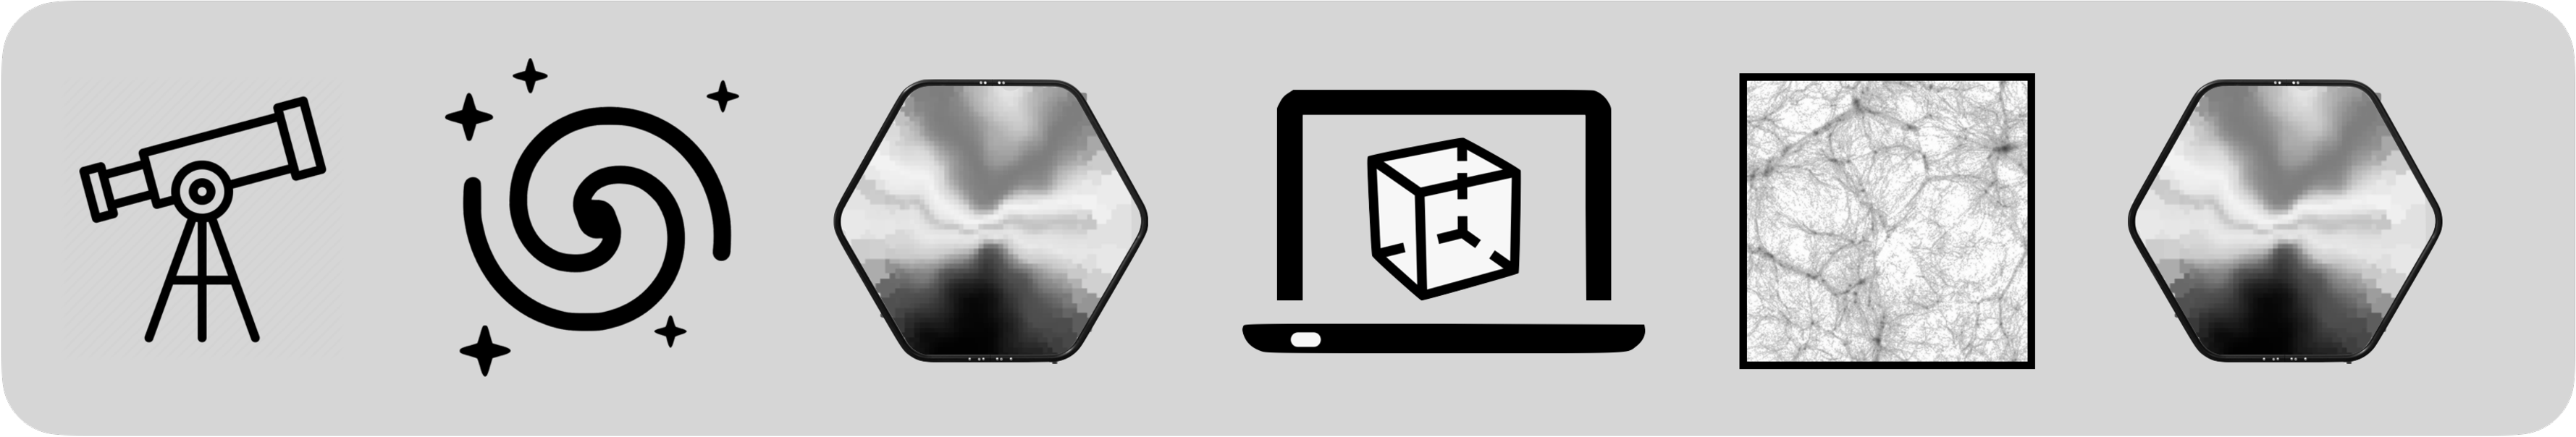
\includegraphics[height=1.21in]{thesis/latex/headers/icons.pdf}
\vspace{3in}

\section{Chapter summaries}
In this thesis, the power of using large-scale integral field spectroscopic surveys and cosmological hydrodynamical simulations \textit{in tandem} was utilised to understand how galaxy kinematics can used as a tool to understand the galaxy-halo connection. We demonstrate the relationship of stellar and gas kinematics with morphology and the angular momentum content of the surrounding dark matter halo \citep{duckworth2020a}, with black hole growth and feedback \citep{duckworth2020b} and vicinity to different features of the cosmic web \citep{duckworth2019}. We also investigate how angular momentum is connected to the large-scale environment in which the galaxy evolves in, demonstrating that galaxies of different morphologies preferentially align with neighbouring filaments (Kraljic, Duckworth et al. in prep.), and that galaxy spin is modulated by vicinity to the nodes (density peaks) and filaments of the cosmic web (Duckworth et al. in prep.). We also demonstrate the potential for a novel application of the axisymmetric Jean's equations in order to recover the underlying dark matter dynamics with the cosmic web. We motivate individual galaxies as tracers for the underlying potential, which aide studies aiming to investigate the relationship between dark matter dynamics (and accretion) and the cosmic web. The key findings of this thesis from each Chapter is as follows:

\begin{itemize}
    \item \textbf{Chapter 2:} We investigate the key relationships of kinematic misalignment (offset rotation between stars and gas) with a galaxy's morphology, stellar angular momentum, gas content, and, spin of the host dark matter halo. We make use of 6000 galaxies from the MaNGA integral field spectroscopic survey to demonstrate that misalignment is much more prevalent in earlier type galaxies, those with lower angular momentum and a lower gas mass (both independent of morphology). We reproduce these trends by creating mock MaNGA observations in the cosmological hydrodynamical simulation of \texttt{IllustrisTNG}, which in turn we use to demonstrate that misalignment can be correlated with lower spin dark matter haloes going back to $z=1$.
    
    \item \textbf{Chapter 3:} We investigate the temporal relationship between kinematically misaligned galaxies and black hole activity in \texttt{IllustrisTNG}. Using the sample of mock MaNGA observations, we demonstrate that low mass misaligned galaxies (identified at $z=0$) have had significantly boosted black hole luminosity, growth and greater feedback (injected into the gas) over the last 8 Gyrs. The epoch of peak energy injection from the black hole feedback is more recent for quenched misaligned galaxies (identified at $z=0$), in comparison to star forming misaligned galaxies. The different persistence timescales of kinematic misalignment versus black hole activity, makes correlation at a single timestep (e.g. $z=0$) difficult in observations.
    
    \item \textbf{Chapter 4:} We investigate how the magnitude and direction of stellar angular momentum of galaxies is modulated by their morphology, stellar mass, and cosmic web environment. We make use of 8000 MaNGA galaxies to determine $\mathrm{\lambda_R}$ (proxy for stellar angular momentum) decreases independently with stellar mass and earlier morphologies. High mass central galaxies (i.e. $\mathrm{M_{stel} > 10^{10.4}M_{\odot}}$) show a dependence on cosmic environment, having lower spins closer to both nodes and filaments. We also determine the three-dimensional alignment between the stellar spin direction of 4000 MaNGA galaxies and their neighbouring filamentary structure of the cosmic web. We demonstrate that the spin of pure LTGs preferentially aligns parallel with the direction of the neighbouring filament, whereas, lenticulars (S0s) preferentially align perpendicular (in both cases driven by the low end of the sample). Kinematically misaligned S0s also particularly show a perpendicular alignment.
    
    \item \textbf{Chapter 5:} We investigate the relationship between kinematic misalignment and large-scale environment, in the context of dark matter halo assembly. We make use of 4000 galaxies in MaNGA to determine that misalignment (used here as a proxy for current gas accretion rate) does not correlate with various halo assembly measures (halo formation time, HOD modelling) and vicinity to cosmic web features at fixed stellar or halo mass. 
    
    \item \textbf{Chapter 6:} We motivate a novel application of the axisymmetric Jeans' equations to recover the three dimensional orbits of galaxies in their surrounding large-scale environment. The velocity anisotropy of dark matter orbits modulates as a function of cosmic environment, and here we demonstrate that so do the galaxies. We introduce a formalism for applying the Jeans' equations to reproduce the velocity anisotropy from stacked potentials of satellites galaxies, with a view to apply this to upcoming spectroscopic surveys such as DESI.
\end{itemize}

\section{Outlook}
This thesis demonstrated the power of using large-scale integral field spectroscopic surveys \textit{in tandem} with cosmological hydrodynamical simulations to understand the galaxy-halo connection. This represents an opportunity to make huge steps forward in building a holistic picture of the angular momentum content of galaxies in the local Universe. MaNGA and SAMI have demonstrated the potential of large-scale IFS surveys, unveiling the diversity of angular momentum content through stellar and gas kinematics, and relationship with fundamental properties such as stellar mass, morphology, and, black hole feedback. Despite this, the exact relationship of the cosmic web with galaxy kinematics is very much an open question. One problem is galaxy sampling, with the completeness and magnitude limit of current large area spectroscopic surveys (such as SDSS) limiting ability to recover all but the largest features of the cosmic web. A second is the typical radial coverage of integral field surveys; since we expect the impact of accretion to be most visible on the outskirts of galaxies, pushing observations to higher radii is crucial in de-convolving signal from internal processes. The future of both redshift and IFS surveys is, however, \textit{bright}.

The Dark Energy Spectroscopic Instrument (DESI) will observe the whole sky, providing a galaxy sample in the local Universe an order of magnitude deeper than SDSS. This will play an integral part of understanding the relationship between the cosmic web and galaxies in the local Universe. In turn, several upcoming IFS surveys are set to go deeper in understanding the role of environment. For example, Hector is the next major dark-time instrument for the Anglo-Australian Telescope and aims to obtain a low-redshift galaxy survey of 15,000 galaxies with IFS observations, with an aim for >70\% imaged out to 2 effective radii. Hector's spectrographs will also have higher spectral resolution than both MaNGA and SAMI, enabling measurements of higher order moments (h3, h4) to link the kinematic tracers to simulations of galaxy merger histories, and, have an more intrincate understand of the accretion history onto the galaxy. 

Another exciting possibility, is the combination of IFS surveys with radio observations to understand the cold gas phases, as a method of identifying fresh gas accretion, potentially from filamentary structure. The HI-MaNGA project; MaNGA galaxies coupled with follow-up radio observation from the Robert C. Bryd Green Bank Telescope (GBT) and archival ALFALFA data will cover up-to 70\% of the completed MaNGA survey \citet{himanga}. In addition, the future survey WEAVE-Apertif (combining radio observations from APERTIF with IFU observations from WEAVE) will yield $\sim10^4$ galaxies with redshifts, neutral gas content, morphologies, dynamics, and dynamical masses. An important distinction of WEAVE-Apertif lies in its HI selection of targets. 

Another pathway in making direct comparisons between observations and simulations, is to extend the comparison to IFS surveys to higher redshifts. One such example, is the upcoming Middle Ages Galaxy Properties with Integral Field Spectroscopy (MAGPI) survey that will observe stellar and gas kinematics for $\sim 60$ central galaxies (and 40+ satellites) at $z\sim0.25-0.35$. The target sample will cover a wide range of halo masses, and will have environmental information from the redshift survey GAMA to better understand the physical processes responsible for the rapid transformation of galaxies in this epoch. Pushing to even higher redshifts (and hence relying only on ionized gas to trace kinematics), various KMOS programs (e.g. KMOS Redshift One Survey \citep[KROSS;][]{stott2016}, KMOS Galaxy Evolution Survey (KGES; Tiley in prep.)) have investigated angular momentum relations for 100s of star forming galaxies at $z=1-2$. An interesting prospect is combining IFS surveys at different epochs \citep[e.g.][]{tiley2019} to understand the evolutionary history of individual galaxy populations over the last $\sim10$Gyrs. 

A number of realistic hydrodynamical simulations are now well established, however, despite their large size ($\sim 100$Mpc$^3$) this is often too small to directly reproduce mock IFS surveys (when approaching $\sim 10000$ galaxies). Our mock MaNGA sample was made at the point in the survey where only $\sim$6000 galaxies had been observed, and finding more unique matches from \texttt{IllustrisTNG100} would have been increasingly difficult. The \texttt{IllustrisTNG} suite of simulations, introduced a 300Mpc$^3$ box to provide a significantly larger galaxy sample, albeit at the cost of an order of magnitude loss in resolution. This issue is particular difficult when trying to construct a mock sample of galaxies with $\mathrm{M_{stel} < 10^{9.5} M_{\odot}}$ where there are only a few hundred stellar particles. Moving forward, advances in software development and computing power will enable larger box sizes, without having to sacrifice particle resolution as much. One such project is \texttt{EAGLE-XL} which will simulate a 300Mpc$^{3}$ periodic cube at the same resolution to their current fiducial 100Mpc$^3$ run. The project is also worth highlighting due to the potential of its \textit{up-scalability}. \texttt{EAGLE-XL} aims to build a new open-source simulation framework, \texttt{SWIFT}, which uses task-based parallelism in order to almost perfectly scale weakly with the number of particles unlike other models such as \texttt{GADGET} or \texttt{GIZMO}. Open-source and highly scalable simulation codes represent the best possibility of realising high resolution and realistic hydrodynamical simulations of vast cosmological scales. In future work, we also aim to relate the angular momentum content of galaxies at $z=0$ (and their corresponding alignment between the spin of the baryons, and, their DM halo) to the angular momentum vectors in the initial conditions (i.e. $z = 127$) of \texttt{IllustrisTNG}.

% NOTE: The \appendix command means that chapters will now change from numbers to letters

\appendix

%\include{appendix_filters}

%\include{appendix_browser}

%\include{appendix_fitter}

%\include{appendix_taurus_data}

%\include{appendix_photometry}

%\include{appendix_catalog}

\backmatter

% NOTE: you can also add pages like the following. Using the empty pagestyle means that it won't count as a chapter (like the declaration, copyright, abstract, ...)

\pagestyle{empty}

\chapter{Online resources}

\begin{footnotesize}

\noindent [1] - \href{http://circumstellardisks.org/}{http://circumstellardisks.org/}

\noindent [2] - \href{http://stardust.jpl.nasa.gov/}{http://stardust.jpl.nasa.gov/}

\noindent [3] - \href{http://gemelli.colorado.edu/~bwhitney/}{http://gemelli.colorado.edu/~bwhitney/}

\end{footnotesize}

\setstretch{1.1}

\newpage

\ \\

\newpage

% NOTE: finally, the bibliography. I used BibTex, hence all references were in references.bib.

\addcontentsline{toc}{chapter}{Bibliography} % Add bibliography to table of contents
\bibliographystyle{apj_tr9} % limits to 8 authors, longer author lists go to et al.
\bibliography{biblio}   % main bib file

\end{document}
